\section{Aufbau und Durchführung}
\label{sec:Durchführung}
 \subsection{Vorbereitung}
  \label{subsec:Vorbereitung}
Bevor der Versuch durchgeführt werden kann,
ist es notwendig das die Resonanzfrequenzen der
beiden Schwingkeise aufeinander abgestimmt werden.
Bei dem Versuchsaufbau existiert ein Schwingkreis
mit konstanter(1) und einer mit variablen(2) Kapazität.
Zu erst muss die Resonanzfrequenz des ersten
Schwingkreises gemessen werden.Dafür wird die Schaltung
wie in Abbildung \ref{abb:messungresonanz} aufgebaut.
\begin{figure}[h]
     \centering
     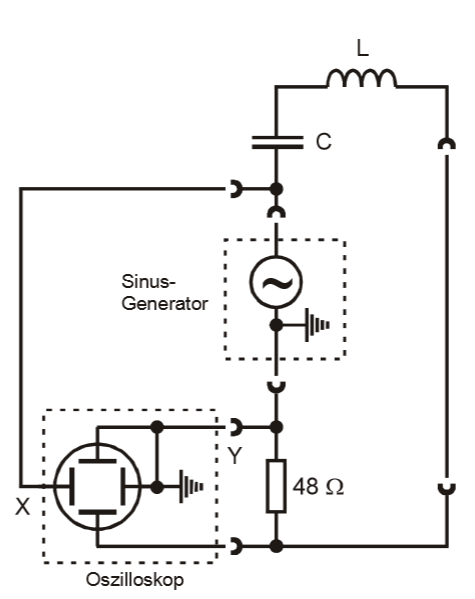
\includegraphics[width=0.5\textwidth]{resonanzbestimmung.PNG}
     \caption{Schaltung zur bestimmung der
     Resonanzfrequenz eines Schwingkreis.\cite{skript} }
     \label{abb:messungresonanz}
\end{figure}\\
Desweiteren wird das Oszilloskop in den X-Y-Betrieb geschaltet und
die Frequenz am Sinus-Generator so geregelt, dass die Lissajous-Figur
eine Gerade ergibt; dies bedeutet das die Frequenz der Resonanzfrequenz des
Schwingkreises entspricht. Die Messung wird nun für den anderen Schwingkreis wiederholt
mit dem Unteschied, dass die Frequenz am Sinus-Generator, die zuvor eingestellt wurde,
konstant bleibt und nur die Kapazität so verändert wird, so dass wieder die Lissajous-Figur
eine Gerade ist. Nun sind beide Resonanzfrequenzen aufeinander abgestimmt und es kann mit
dem Versuch begonnen werden.
\subsection{Durchführung}
\label{subsec:Durchführung}
Für die Versuchsdurchführung wird nun die Schaltung
wie in Abbildung \ref{abb:schwebungsaufbau} aufgebaut.
\begin{figure}[h]
   \centering
   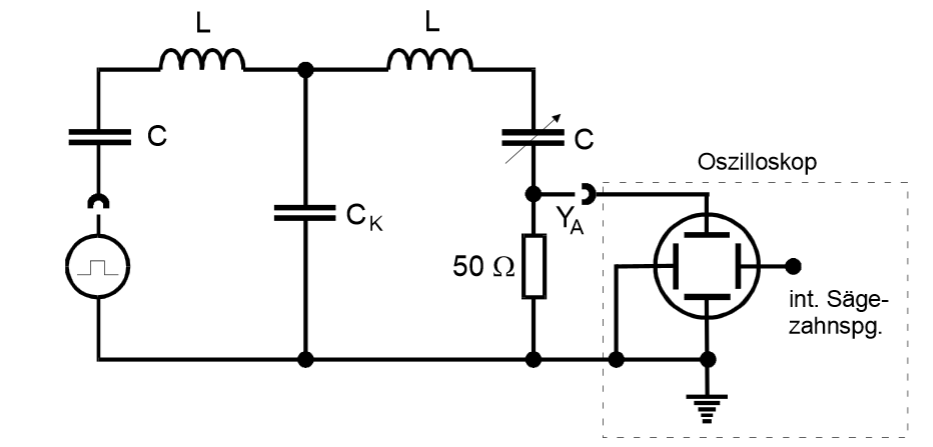
\includegraphics[width=0.9\textwidth]{Aufbau_a).PNG}
   \caption{Schaltung zur Untersuchung von Schwebungen bei gekoppelten Schwingkreisen \cite{skript}}
   \label{abb:schwebungsaufbau}
\end{figure}\\
Nun wird mit einer Rechteckspannung der
Schwingkreis 1 erregt, hier bei ist die anregende Frequenz
deutlich geringer als die Resonanzfrequenzen.
Dieser ist über den Koppelkondensator,
variabler Kapazität$C_k$, mit dem anderen Schwingkreis 2
verbunden. Am Schwingkreis 2 wird mit
Hilfe eines Ozilloskopes die Spannung aufgezeichnet.
Das Ozilloskop zeigt eine Schwebung, wo nun das Verhältnis
zwischen Schwingugs- und Schwebungsfrequenz aufgenommen wird.
Dies wird für unterschiedliche $C_k$ wiederholt.
\\
Desweiteren werden die Fundamentalfrequenzen
in Abhängigkeit von $C_k$
des gekoppelten Schwingkreises gemessen.
Hier für wird der Rechteck- durch
eine Sinusgenerator ausgetauscht und außerdem
noch mit anderen Eingang des Oszilloskop verbunden(\ref{abb:fundamentalaufbau})
\begin{figure}[h]
  \centering
  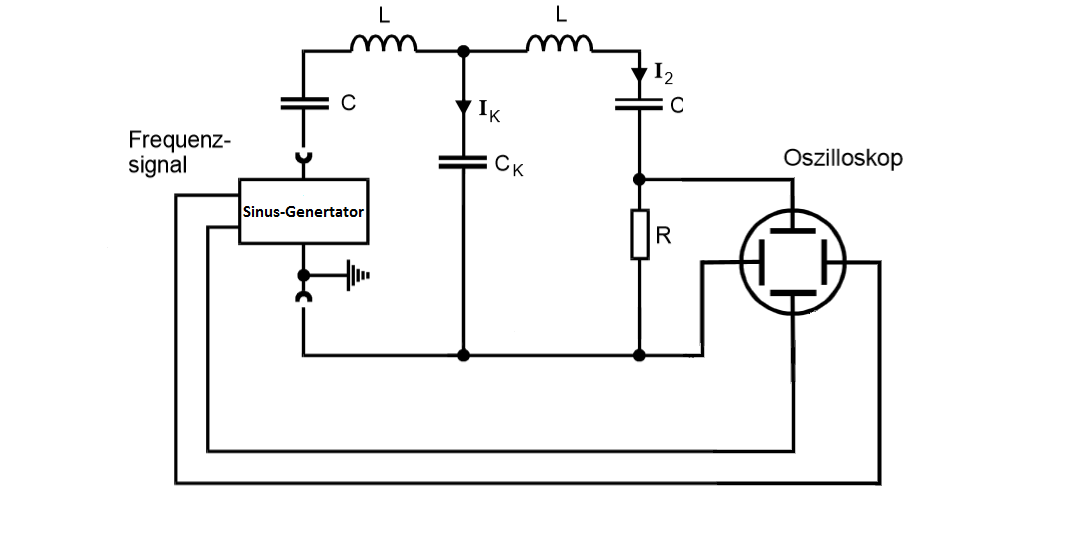
\includegraphics[width=0.7\textwidth]{physik.PNG}
  \caption{Schaltung zur Untersuchung von Fundamentalfrequenzen bei gekoppelten Schwingkreisen \cite{skript}}
  \label{abb:fundamentalaufbau}
\end{figure}\\
Die Frequenz des Sinusgenerators wird um
die in dem Kapitel \ref{subsec:Vorbereitung}
gemessenen Frequenzen variiert.
Das Oszilloskop wird wieder im X-Y-Betrieb benutzt
und eine Fundamentalfrequenz lässt sich messen
, wenn die Lissajous-Figur eine Gerade ist.
Dies geschied zweimal, da es einmal $\nu^+$ und
$\nu^-$ gibt. Dies wurde hierbei aber nicht mit den Lissajour-Figuren gemessen
sondern in dem durch leichtes Verstellen der Frequenz, die Frequenzen ausgewählt wurde wo die Amplitude maximal war.
Somit wurde auch deutlich ob es sich um $\nu^+ $ oder $\nu^-$ handelte.   \\
\\
Die Fundamentalfrequenzen lassen sich
ebenfalls durch das Frequenzspektrum ermitteln.
Dafür wird der Sinus-Generator
aus Abbildung \ref{abb:fundamentalaufbau}
in den Sweepmodus geschaltet.
Der Sweep wird so eingestellt, dass dieser unterhalb
der in der Vorbereitung \ref{subsec:Vorbereitung}
gemessenen Frequenzen anfängt
und oberhalb aufhört.
Das Oszilloskop nimmt den Spannungsverlauf des
2. Schwingkreises auf. Die zwei Hochpunkte sind die
beiden Fundamentalfrequenzen, wo der zeitlich
Abstand zum Sweepanfang gemessen wird.
Dies wird  für die anderen Kapazitäten wiederholt.\\

\subsection{Eigenschaften der Bauteile}
Für die Messungen werden Bauteile mit folgenden Eigenschaften eingesetzt:
\begin{align*}
\text{Induktivität der Spule:} \  L&=23,954\si{\micro\henry}\\
\text{Kapazität des Kondensators:} \  C&=0,7932\si{\nano\farad}\\
\text{Kapazität der Spule:} \ C_{Sp}&=0,028\si{\nano\farad}\\
\end{align*}\\
\begin{table}
  \centering
  \caption{Kapazitäten des Koppelkondensators}
  \label{tab:koppelkondensator}
  \begin{tabular}{c}
    \toprule
    $C_k \ \mathrm{in} \ \si{\nano\farad}$ \\
    \midrule
    1,0 \\
    2,2 \\
    2,7 \\
    4,7 \\
    6,8 \\
    8,2 \\
    10,0 \\
    12,0 \\
    \bottomrule
   \end{tabular}
\end{table}
